\documentclass{report}[pt12]
\usepackage{amsmath}
\usepackage{tikz}
\usepackage[section]{placeins}
\usepackage{hyperref}

\hypersetup{
colorlinks,
citecolor=black,
filecolor=black,
linkcolor=black,
urlcolor=black
linkto=all,
}
\usetikzlibrary{automata, arrows.meta, positioning}

\title{Language and Automata, Assignment 2}
\author{Krzysztof Rudnicki\\ Student number: 307585}
\date{\today}


\begin{document}
\maketitle

\chapter{Regular expression}
We are given following regular expression:
\[ 0^n1^m2^m3^n \]

\chapter{Diagram of the automata}
I used the following notation for transitions:
I, S / $N_S$
Where: \\
I - Input from the string \\
S - Element currently on top of the stack \\
/ - a dash to make it easier to differentiate between \emph{before} transition and \emph{after} \\
$N_S$ - How the top of the stack will look after the transiton, if there are 2 symbols read it like this: leftmost symbol will be on top of the stack as a new symbol, rightmost symbol is just below this symbol, I use this to denote that I am NOT deleting the earlier symbol from stack, if there is 1 symbol it means that this symbol will be on top of the stack, if there is $\epsilon$ it means that I pop (remove) the symbol from top of the stack.


\begin{figure}[!htb]
\centering
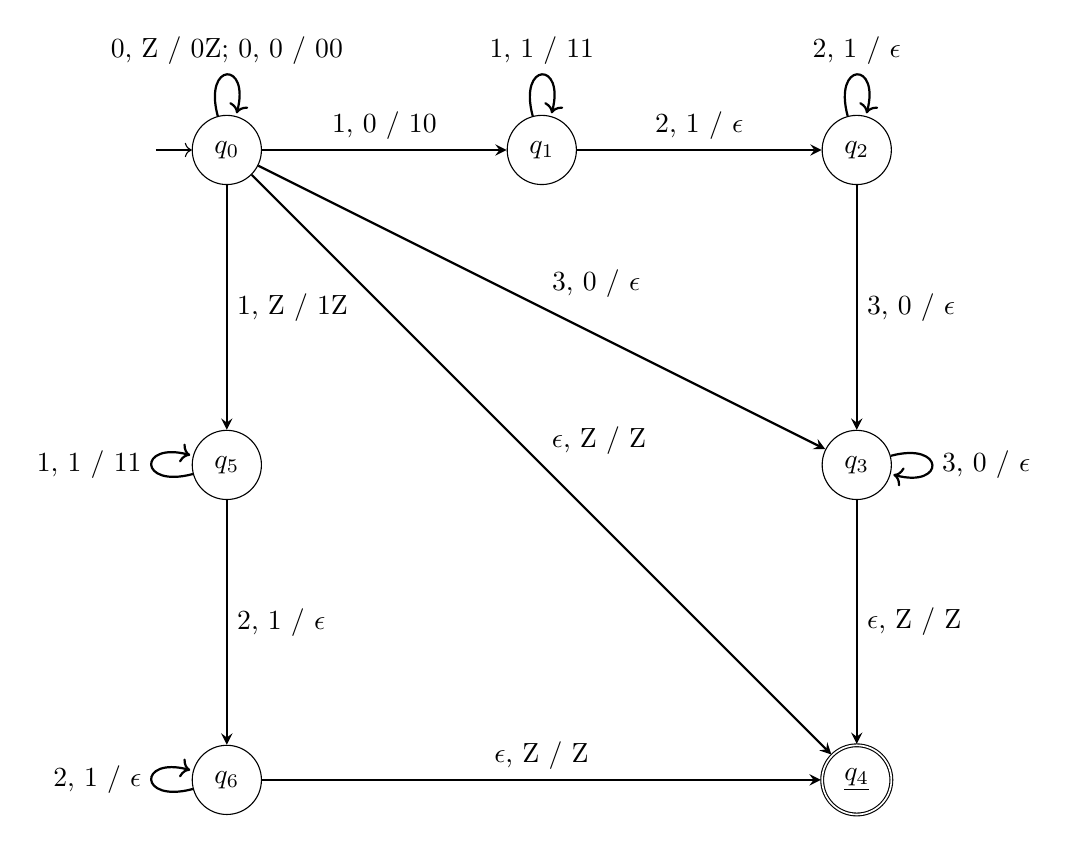
\begin{tikzpicture} [node distance = 4cm, on grid, auto]

\node (q0) [state, initial, initial text = {}] {$q_0$};
\node (q1) [state, right = of q0] {$q_1$};
\node (q2) [state, right = of q1] {$q_2$};
\node (q3) [state, below = of q2] {$q_3$};
\node (q4) [state, accepting, initial text = {}, below = of q3] {$\underline{q_4}$};
\node (q5) [state, below = of q0] {$q_5$};
\node (q6) [state, below = of q5] {$q_6$};

\path [-stealth, thick]
    (q0) edge [loop above] node {0, Z / 0Z; 0, 0 / 00 }   (q0);
  \path [-stealth, thick]
      (q0) edge node {1, 0 / 10}   (q1);
  \path [-stealth, thick]
      (q1) edge [loop above] node {1, 1 / 11}   (q1);
  \path [-stealth, thick]
      (q1) edge node {2, 1 / $\epsilon$}   (q2);
  \path [-stealth, thick]
      (q2) edge [loop above] node {2, 1 / $\epsilon$}   (q2);
  \path [-stealth, thick]
      (q2) edge node {3, 0 / $\epsilon$}   (q3);
  \path [-stealth, thick]
      (q3) edge [loop right] node {3, 0 / $\epsilon$}   (q3);
  \path [-stealth, thick]
      (q3) edge node {$\epsilon$, Z / Z}   (q4);
  \path [-stealth, thick]
      (q0) edge node {1, Z / 1Z}   (q5);
  \path [-stealth, thick]
      (q5) edge [loop left] node {1, 1 / 11}   (q5);
  \path [-stealth, thick]
      (q5) edge node {2, 1 / $\epsilon$}   (q6);
  \path [-stealth, thick]
      (q6) edge [loop left] node {2, 1 / $\epsilon$}   (q6);
  \path [-stealth, thick]
      (q6) edge node {$\epsilon$, Z / Z}   (q4);
\path [-stealth, thick]
    (q0) edge node {3, 0 / $\epsilon$}   (q3);
\path [-stealth, thick]
      (q0) edge node {$\epsilon$, Z / Z}   (q4);

\end{tikzpicture}
\caption{Diagram of the automata} \label{fig:diagram}
\end{figure}

\chapter{Description of states and the behaviour of PDA}
\section{Cases}
I recognized 4 possible cases for this automata:
\begin{enumerate}
\item m = 0
Our input string will look like this: $0^n3^n$. If we encounter something like this we should keep pushing 0's to the stack until we encounter 3. Once we receive 3, we check if on top of the stack we have 0 and then pop it from stack. Then we can either empty the stack and run out of 3's and which point we go to the accepting state, otherwise we go to the fail state, we go to the fail state if:
\\ We run out of 3's before we run out of 0 (number of 3 is smaller than number of 0)
\\ We run out of 0's before we run out of 3 (number of 3 is bigger than number of 0)
I will refer to the
\[ q_0 \rightarrow q_3 \rightarrow \underline{q_4} \]
path, as the case 1 route
\item n = 0
We will do exactly the same as in example above but swap 0 with 1 and 3 with 2.
I will refer to the
\[ q_0 \rightarrow q_5 \rightarrow q_6 \rightarrow \underline{q_4} \]
path, as the case 2 route
\item n, m $>$ 0
Our input string will look like this: $0^n1^m2^m3^n$.
First we push 0's and 1's on stack. Once we encounter 2 we check if we have 1 on top of the stack, then pop it. We keep popping 1's until we run out of 2's. Then once we encounter 3 we check if we have 0's on top of the stack and keep popping 0's until we run out of 3's. If stack is empty by the end of the string we move to the accepting state, otherwise we move to the fail state.

I will refer to the
\[ q_0 \rightarrow q_1 \rightarrow q_2 \rightarrow q_3 \rightarrow \underline{q_4} \]
path, as the case 3 route
\item n = 0, m = 0
String will be empty but also accepted by this grammar. In this case we will just go straight to the accepting state.
I will refer to the
\[ q_0 \rightarrow \underline{q_4} \]
path, as the case 3 route
\end{enumerate}

\section{Notes on behaviour and design decisions}
\subsection{Non-deterministic}
I decided to make non-deterministic PDA since it was much easier as it allowed me to deconstruct the problem on the case basis, if you take a look at the "route" below the starting state, this is the route that corresponds to case number 2, where n = 0. This was very easy to implement since I used non-deterministic PDA.

\subsection{Accepting by non-empty stack}
I also decided to make this PDA accepting by empty stack, I use the letter 'Z' to denote start symbol so empty stack, notice that when: \\
I get 0 at the start state I put this 0 on stack - case 1 and 3
Later when I get epsilon from input I check if I am on 'Z' on stack and go to the accepting state \\
I get 1 at the start state I put this 1 on stack - case 2
Later when I get epsilon from input I check if I am on 'Z' on stack and go to the accepting state \\
I get $epsilon$ at the start state I do not put anything on stack and go to the final state - case 4 \\
I decided to use PDA accepting by empty stack since it was easier to create since it allowed for easier design of pushing and popping equal number of symbols on stack.

\section{Description of states}
\begin{itemize}
\item $q_0$ - Starting state, based on the input we get from string it decides whether we go down the case 1 route (0 then 3 on input), case 2 route (1 on input), 3 route (0 on input) or case 4 route ($\epsilon$ on input).
\item $q_1$ - State in which we keep on pushing 1 on stack from input, once we receive 2 we move onto state $q_2$
\item $q_2$ - State in which we keep pushing 2 on stack from input, once we receive 3 we move onto state $q_3$
\item $q_3$ - State in which we keep \emph{popping} 0 from stack if we receive the 3 from input, once the input is empty \textbf{AND} we have accepting symbol on stack we move to the accepting $\underline{q_4}$ state
\item $\underline{q_4}$ - Accepting state, there is no moving out of this state since we checked that the input is already empty
\item $q_5$ - This state is accessible if we went down case 2 route, we keep on pushing 1 from input to stack and once we receive 2 we go to the $q_6$ state
\item $q_6$ - This state is accessible if we went down case 2 route, we keep on \emph{popping} 1 from stack if we receive 2 and once the input is empty \textbf{AND} and we have accepting symbol on top of the stack we move to the accepting $\underline{q_4}$ state.
\end{itemize}

\section{PDA description}
I will describe PDA as:
\[ M = \{Q, \sum, \Gamma, \delta, q_0, Z_0, F \} \]
Where:
Q - set of states
\[ Q = \{q_0, q_1, q_2, q_3, \underline{q_4}, q_5, q_6\} \]
$\sum$ - Input alphabet
\[ \sum = \{0, 1, 2, 3 \} \]
$\Gamma$ - Stack Alphabet
\[ \Gamma = \{ 0, 1, Z \} \]
$\delta$ - transition function
You can find them \hyperlink{transition}{\textbf{here}}:
$q_0 = q_0$ - start state
$Z_0 = Z$ - start symbol
$F = q_4$ - final states



\hypertarget{transition}{\chapter{Transition functions}}
Write the transition function (as triplets…).
\[ \delta(q_0, 0, Z) = (q_0, 0Z) \]
\[ \delta(q_0, 0, 0) = (q_0, 00) \]
\[ \delta(q_0, 1, 0) = (q_1, 10) \]
\[ \delta(q_0, 3, 0) = (q_3, \epsilon) \]
\[ \delta(q_0, 1, Z) = (\underline{q_4}, Z) \]
\[ \delta(q_1, 1, 1) = (q_1, 11) \]
\[ \delta(q_1, 2, 1) = (q_2, \epsilon) \]
\[ \delta(q_2, 2, 1) = (q_2, \epsilon) \]
\[ \delta(q_2, 3, 0) = (q_3, \epsilon) \]
\[ \delta(q_3, 3, 0) = (q_3, \epsilon) \]
\[ \delta(q_3, \epsilon, Z) = (\underline{q_4}, Z) \]
\[ \delta(q_5, 1, 1) = (q_5, 11) \]
\[ \delta(q_5, 2, 1) = (q_6, \epsilon) \]
\[ \delta(q_6, 2, 1) = (q_6, \epsilon) \]
\[ \delta(q_6, \epsilon, Z) = (\underline{q_4}, Z) \]

\chapter{Instantaneous description accepting example}
$\epsilon$
\[ (q_0, \epsilon, Z) \vdash (\underline{q_4}, \epsilon, Z) \]
03 string
\[ (q_0, 03, Z) \vdash (q_0, 3, 0Z) \vdash (q_3, \epsilon, Z) \vdash (\underline{q_4}, \epsilon, Z) \]
12 string
\[ (q_0, 12, Z) \vdash (q_5, 2, 1Z) \vdash (q_6, \epsilon, Z) \vdash (\underline{q_4}, \epsilon, Z) \]
001233 string
\[ (q_0, 001233, Z) \vdash (q_0, 01233, 0Z) \vdash (q_0, 1233, 00Z) \vdash (q_1, 233, 100Z) \vdash (q_2, 33, 00Z) \vdash (q_3, 3, 0Z) \vdash (q_3, \epsilon, Z) \]
\[ \vdash (\underline{q_4}, \epsilon, Z) \]
\chapter{Instantaneous description rejecting example}
\[ (q_0, 0, Z) \vdash (q_0, \epsilon, 0Z) \]
There is no transition for state $q_0$, $\epsilon$ on input and 0 on top of stack so the string gets rejected
\[ (q_0, 0012333, Z) \vdash (q_0, 012333, 0Z) \vdash (q_0, 12333, 00Z) \vdash (q_1, 2333, 100Z) \vdash (q_2, 333, 00Z) \vdash \]
\[ (q_3, 33, 0Z) \vdash (q_3, 3, Z) \]
There is no transition for $(q_3, 3, Z)$ so the string gets rejected
\[ (q_0, 033, Z) \vdash (q_0, 33, 0Z) \vdash (q_3, 3, Z) \]
There is no transition for $\vdash (q_3, 3, Z)$ so the string gets rejected
\[ (q_0, 122, Z) \vdash (q_5, 22, 1Z) \vdash (q_6, 2, Z) \]
There is no transition for $(q_6, 2, Z)$ so the string gets rejected

\end{document}
